\title{Neuronal Connectivity via \\Bayesian Tensor Factorization}
\author{Chris Mulligan}
\date{December 18, 2015}

% ****************************************************************************
% Document Start
\documentclass{article}


\usepackage[T1]{fontenc}
\usepackage{amsmath}
\usepackage{amsfonts}
\usepackage{hyperref}
\usepackage[square,numbers]{natbib}
\bibliographystyle{ieeetr}
\usepackage{epsfig}
\usepackage{url}
\usepackage{bm}

\newcommand{\tensor}[1]{\ensuremath{\underline{\mathbf{#1}}}}


\begin{document}
\maketitle

\section{Introduction}
\label{sec:intro}
In modern statistical neuroscience there is significant interest in discovering and modeling connections between individual neurons. The connections between neurons are useful for understanding how neurons process information and compute.

Recent advances in calcium imaging and multielectrode arrays give us access to the simultaneous spike train data for hundreds, or potentially even thousands, of neurons. Although with a few exceptions, such as C. elegens, this represents only a small fraction of the neurons in an organism, the techniques now employed are still quite valuable.

Parallel to this development in neuroscience, machine learning has seen a surge in development of, and interest in, matrix factorization techniques. While Non-negative matrix factorization (NMF) has been in use for many years, with the recent availability of very large dyadic datasets, many from internet companies like Netflix, there's been strong appreciation for NMF. More recently there's been interest in extending NMF from the 2 way regime of matrices to the M way regime of tensors. Along with these decomposition techniques, advances in inference algorithms, particularly Variational Inference and efficient MCMC algorithms, have allowed machine learning users to fit larger and more complex Bayesian models.

In this work we apply the techniques of probabilistic tensor factorization to the problem of neuron connectivity. While currently this technique does not provide strictly more accurate answers than other methods, it provides an interesting new avenue for exploratory data analysis and visualization.  

There has been a significant amount of interest and prior work in neuron connectivity. Classically Cross-Correlation and Granger Causality based techniques were employed \cite{perkel1967neuronal,kaminski2001evaluating} Generalized Linear Models \cite{paninski2004maximum}.  More recently Generalized Linear Models,  particularly $L_1$-regularized GLMs, have been applied with quantitative success, although the models don't lend themselves to interpretability as well as other techniques \cite{paninski2004maximum,zhao20121}. A promising, though also problematic, literature is developing around network Hawkes processes, which can leverage some of the work in GLMs but offers advantages in inference and interpretability \cite{linderman2015scalable}. Perhaps the most similar work is recent applications of clustered factor analysis techniques to spike data \cite{buesing2014clustered}, although there's other very current work applying factorization techniques to neural data \cite{rudolph2015,friedrich2015}.


% *********************************************
\section{Bayesian Tensor Factorization}
\label{sec:btf}
\subsection{Model Definitions}
\label{sec:model}
We consider a standard setup with multiple simultaneously recorded spike trains. This consists of dataset of $y_{it}$, the observed spike count for neuron $i=1,\ldots,N$ during time step $t=1,\ldots,T$. 

We will consider looking at neuron firings over a set of lags, some small number time steps over which we will infer the neuron interactions. Let $L \ll T$ be the maximum lag we consider. 

Let $\tensor{Y}$ be a three way tensor of size $N \times N \times L$. Each element $y_{ijl} \in \mathbb{Z}_{\geq 0}$ is the count of times that neuron $i$ fired $l$ time steps after neuron $j$. This creates a triadic dataset, which describes the pairwise associations between neurons over a sliding window of up to $L$ times, centered at each firing of the neuron.

As we see in the results in section~\ref{sec:connectomics}, the formulation discussed here is not without its problems. In section~\ref{sec:future} we propose an alternative model where $y_{ijl} \in [0, 1]$ is the conditional probability of neuron $i$ firing $l$ time steps after neuron $j$. While conceptually similar, it introduces additional mathematical and inferential difficultly. 

\subsection{Tensor Factorization}
\label{sec:factorization}
We use the Canonical Polyadic (CP) decomposition, because compared to the common alternative Tucker decomposition it is more interpretable and performs better with sparse counts \cite{schein2015bayesian,kolda2008scalable}. The $K$ component decomposition decomposes the 3 way tensor into 3 latent factor matrices $\Theta^{(1)}, \Theta^{(3)}, \Theta^{(2)}$, with dimensions $d_m \times K$. 

$$y_{ijl} \approx \hat{y}_{ijl} = \sum_{k=1}^K \theta^{1}_{ik} \theta^{2}_{jk} \theta^{3}_{lk}$$

Frequently $\hat{y}_{ijl}$ is called the ``reconstruction'' $y_{ijl}$, and represents the estimate based on the decomposition.

The columns of each of the $\Theta$ matrices represent a latent \textit{component}, which hopefully will indicate a meaningful relationship between neurons. 
The $\Theta^{(1)}_k$ vector represents the neurons being ``predicted'',
while the $\Theta^{(3)}_k$ vector represents the neurons being depended on, and 
$\Theta^{(2)}_k$ represents the lags of the dependency.


\subsection{Probabilistic Model}
\label{sec:bayesian}
We can interpret the deterministic decomposition in a probabilistic lens, where the reconstruction is the expected value of a distribution for the actual observed data. In this case we consider $y$ a Poisson random variable, although other distributions are feasible, such as the Bernoulli conjectured in section~\ref{sec:future}. Thus:

$$y_{ijl} \sim Pois(\hat{y}_{ijl})$$

With this framework we can use maximum likelihood estimation using the poisson likelihood for the $\Theta$ matrices, which yields superior results to using squared error, and implicitly assuming a Gaussian likelihood. However, we can do even better than MLE with Poisson likelihood by using a Bayesian inference, following the work of Schein et al which generalizes Poisson Matrix Factorization to Tensors \cite{cemgil2009bayesian,schein2015bayesian,ermics2015link}. 

The conjugate prior for the Poisson distribution is the Gamma, and it has certain other nice properties for our purposes, therefore we impose the prior $\theta_{ik}^{(m)} \sim \textrm{Gamma}(\alpha, \alpha \beta^{(m)})$. Under this parameterization we take a very small $\alpha$ and small(ish) $\beta$, as seen in figure~\ref{fig:gamma}, which concentrates the probability mass near 0, but has a heavy tail. This prior naturally encourages the desired sparsity in the latent factors. The $\alpha$ value is set manually, and in the style of empirical Bayes $\beta$ is estimated as part of the inference, since $1/\beta^{(m)}$ is the mean of $\Theta^{(m)}$. 

\begin{figure}[!b]
\centering
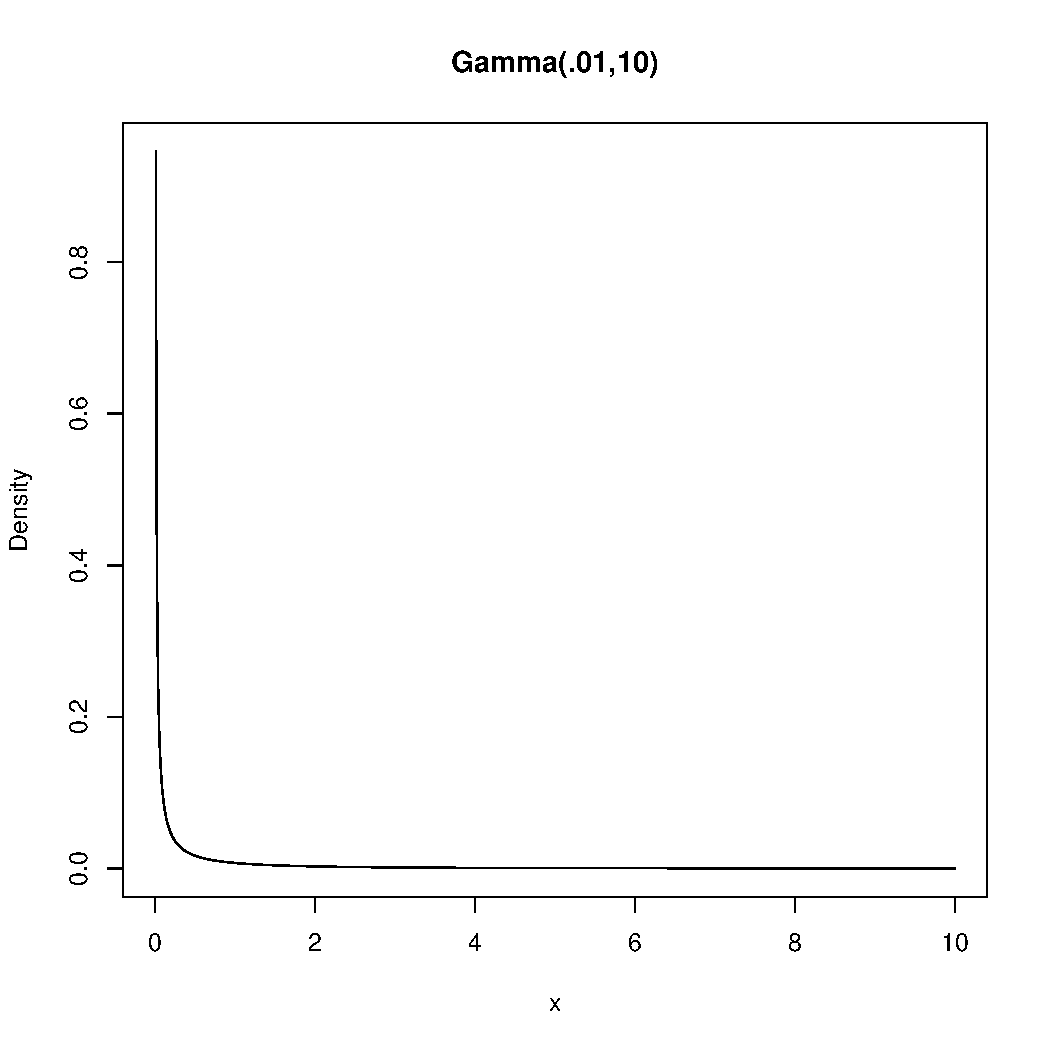
\includegraphics[width=.5\linewidth]{gamma}
\caption{Gamma(.01, 10) Density}
\label{fig:gamma}
\end{figure}



\subsection{Approximate Inference}
\label{sec:inference}
The posterior distribution is:

$$P\left(\Theta^{(1:3)} \ |\  \tensor{Y}, \alpha, \beta^{(1:3)} \right)$$

As with most models, this posterior is analytically infeasible, and therefore must be approximated. We use standard variational inference techniques using a mean field approximation, based on the Python code released by Schein et al \cite{schein2015bayesian}. In variational inference we posit a family of distributions $Q$, with parameters $S = \{\gamma_{d_m \cdot k \cdot m}, \delta_{d_m \cdot k \cdot m} \}$. Then solve the optimization problem $S^* = \textrm{argmin}_S \textrm{KL}(P || Q)$, to choose the member of $Q$ as similar as possible to the posterior.

Here because the $Q$ distribution factorizes completely the optimization can be done via coordinate ascent, using convergence of the evidence lower bound (ELBO) as the stopping criteria, where the ELBO is:

$$\mathcal{B}(S) = \mathbb{E}_Q\left[\log P(\tensor{Y}, \Theta^{(1:3)}|\alpha, \beta^{(1:3)})\right] + H(Q)$$

We use independent Gamma variables for each latent factor, eg:

$$P\left(\theta^{(1)}_{ik}|\cdot\right) \approx Q\left(\theta^{(1)}_{ik} | S^{(1)}_{ik}\right) = \textrm{Gamma}\left(\theta^{(1)}_{ik} | \gamma^{(1)}_{ik}, \delta^{(1)}_{ik}\right)$$

As derived in Bayesian Poission Matrix Factorization \cite{cemgil2009bayesian} and Tensor Factorization \cite{schein2015bayesian}, the update equations are, eg:

$$\gamma_{ik}^{(1)} = \alpha + \sum_{j, l} y_{ijl} \frac{\mathbb{G}_Q\left[ \theta_{ik}^{(1)} \theta_{jk}^{(2)} \theta_{lk}^{(3)} \right]}{\sum_{k=1}^K \mathbb{G}_Q\left[ \theta_{ik}^{(1)} \theta_{jk}^{(2)} \theta_{lk}^{(3)} \right]}  = \alpha + \sum_{j, l} y_{ijl} \frac{\mathbb{G}_Q\left[ \theta_{ik}^{(1)} \right] \mathbb{G}_Q\left[\theta_{jk}^{(2)}\right] \mathbb{G}_Q\left[\theta_{lk}^{(3)} \right]}{\sum_{k=1}^K \mathbb{G}_Q\left[ \theta_{ik}^{(1)} \right] \mathbb{G}_Q\left[\theta_{jk}^{(2)}\right] \mathbb{G}_Q\left[\theta_{lk}^{(3)} \right]}$$

$$\delta_{ik}^{(1)} = \alpha\beta^{(1)} + \sum_{j,l} \mathbb{E}_Q \left[ \theta_{ik}^{(1)} \theta_{jk}^{(2)} \theta_{lk}^{(3)} \right] = \alpha\beta^{(1)} + \sum_{j,l} \mathbb{E}_Q\left[ \theta_{ik}^{(1)} \right] \mathbb{E}_Q\left[\theta_{jk}^{(2)}\right] \mathbb{E}_Q\left[\theta_{lk}^{(3)} \right]$$

This lends itself to numerous computational tricks for efficient inference, including memoizing the individual expectations and the denominator of $\gamma$, and not calculating any of the expectations for $\gamma$ in the case that $y_{ijl} = 0$.


% *********************************************
\section{Results}
\label{sec:results}

\subsection{Simple Synthetic Result}
\label{sec:simple}
A small synthetic dataset consisting of 25 integrate and fire simulated neurons over 100,000ms was constructed with EnaS, simulating Multi-Electrode Array data \cite{nasser2013enas}. Implanted within these neurons were approximately 5 very strong connections with varying lag times, and standard connections otherwise. From this raw data we construct our tensor $\tensor{Y}$ with $L=20$ maximum lag. This tiny dataset yields a tensor with $25\times25\times20 = 12,500$ values.

\begin{figure}[!ht]
\centering
\begin{tabular}{cc}
\includegraphics[width=.5\linewidth,page=1]{../enas_sim1_raster_unit-time.out/45_trained_model.pdf} & \includegraphics[width=.5\linewidth,page=2]{../enas_sim1_raster_unit-time.out/45_trained_model.pdf} \\
\includegraphics[width=.5\linewidth,page=3]{../enas_sim1_raster_unit-time.out/45_trained_model.pdf} & \includegraphics[width=.5\linewidth,page=4]{../enas_sim1_raster_unit-time.out/45_trained_model.pdf} \\
\includegraphics[width=.5\linewidth,page=5]{../enas_sim1_raster_unit-time.out/45_trained_model.pdf} & \includegraphics[width=.5\linewidth,page=6]{../enas_sim1_raster_unit-time.out/45_trained_model.pdf} 
\end{tabular}
\caption{Our 6 fitted components for the Simple Synthetic Data}
\label{fig:simple}
\end{figure}


We employ the tensor factorization procedure described here with $K=6$ components and $\alpha = .01$. The components are visualized in figure~\ref{fig:simple}. Each sub-figure consists of a component, and within the components the top left plot displays the weights on the triggered neurons, while the top right displays the weights on the triggering neurons, and the lower section visualizes the lags over which that interaction occurs.

Notice that in component 3 (labeled ``G2'', middle row, left side) neuron 5 depends strongly on neuron 21, with a lag of 2. In component 2 (labeled ``G1'', top right), there's a more complicated relationship where neurons 9, 11, 19, and 24 depend primarily on neuron 3, but also neuron 20, with a lag of 3. 

There are several sensible ways of deriving a directed graph $\hat{W}$ from the factorization. Most intuitively, we can sum out the time dimension, and get $\hat{w}_{ij} = \sum_{l=1}^L \hat{y}_{ijl}$. Alternatively, we can examine the product of the first two latent dimensions, $\Theta^{(1)} \Theta^{(2)\textrm{T}}$, visualized in figure~\ref{fig:dot_product}. 

\begin{figure}[!h]
	\centering
	\includegraphics[width=.4\linewidth,page=7]{../enas_sim1_raster_unit-time.out/45_trained_model.pdf}
	\caption{Simple Synthetic Data connectivity graph inference}
	\label{fig:dot_product}
\end{figure}

From this data we can see that, given a very small network with clean and strong interactions this technique recovers those interactions. The latent components derived lend themselves well to visualization and interpretation. This suggests that this method is promising. However, this dataset is very small and very clean, so we need to proceed to more realistic settings. 


\subsection{Connectomics Challenges Results}
\label{sec:connectomics}
We consider the ``realistic'' synthetic data provided by the Connectomics Challenge \cite{stetter2012model}. They simulate spiking neurons using the NEST simulator\cite{Gewaltig:NEST}, with realistic dynamics and connectivity, then model calcium fluorescence and provide fluorescence data. The specific dataset of theirs I consider has $N=100$ neurons, with $T\approx 180,000$ in a highly clustered network.

I begin by deconvolving the fluorescence to a spike train using the Vogelstein et al , as implemented in the PyFNND package \cite{vogelstein2010fast,pyfnnd}

The dataset was constructed with $L=150$ maximum lag, and fit with $K=50$ components.

\begin{figure}[!h]
\centering
\includegraphics[width=.4\linewidth,page=4]{../fluorescence_iNet1_Size100_CC04inh.out/3_trained_model.pdf}
\caption{Component 3, one of several which captures neuron correlations in ~time 0}
\end{figure}


\begin{figure}[!h]
\centering
\includegraphics[width=.7\linewidth,page=4]{../fluorescence_iNet1_Size100_CC04inh.out/3_trained_model.pdf}
\caption{3: one of several which captures neuron correlations in ~time 0}
\end{figure}

\begin{figure}[!h]
\centering
\includegraphics[width=.7\linewidth,page=32]{../fluorescence_iNet1_Size100_CC04inh.out/3_trained_model.pdf}
\caption{31: Interesting temporal pattern, and sparse $i$ vector}
\end{figure}

\begin{figure}[!h]
\centering
\includegraphics[width=.7\linewidth,page=22]{../fluorescence_iNet1_Size100_CC04inh.out/3_trained_model.pdf}
\caption{21: Note sparsity  of neurons, but relative flatness in time}
\end{figure}

Unfortunate Graph Results
\begin{figure}[h]
\centering
\includegraphics[width=.4\linewidth,page=51]{../fluorescence_iNet1_Size100_CC04inh.out/3_trained_model.pdf}
\hfill
\includegraphics[width=.4\linewidth,page=1]{../network_iNet1_Size100_CC04inh.pdf}
\caption{Left: Inferred with same method. Right: Actual}
\end{figure}

\section{Future Work}
\label{sec:future}

\newpage
\bibliography{neural}


\end{document}
